
\cvsection{Education}
\cvevent{Computer Science - 4.0 GPA}{University of Toronto}{ September 2022 -- Currently}{}
Extracurriculars: Singer in four choirs,\\
debate winner for AI ethics event
% \cvachievement{\faTrophy}{}{Received accolades at Atos for Best Performance in team.}
% \cvachievement{\faTrophy}{}{Received Best Debut Award at Atos. }
% %\divider
% \cvachievement{\faInstitution}{}{Won 2nd Consolation Prize for paper presented on Cognitive Radio Networks.}
% %\divider
% \cvachievement{\faGraduationCap}{}{Got Selected in "Exclusive Scholar Program" during undergrad.}
% %\divider
% \cvachievement{\faDollar}{}{Awarded with Narotam Sekhsaria Foundation Scholarship}
%\cvsection{Strengths}

%\cvtag{Hard-working (18/24)} 
%\cvtag{Persuasive}
%\cvtag{Motivator \& Leader}

%\divider\smallskip

%\cvtag{UX}
%\cvtag{Mobile Devices \& Applications}
%\cvtag{Product Management \& Marketing}


%\divider

%\cvevent{B.S.\ in Symbolic Systems}{Stanford University}{Sept 1993 -- June 1997}{}

\cvsection{Personal Projects}
All projects can be found on my GitHub, linked in the header.

\smallskip
\smallskip
\cvproject{RPSOnline: Online Multiplayer Rock, Paper, Scissors}
\begin{itemize}
\item Backend written in Rust, frontend written in JavaScript, uses a MySQL database
\item Uses Websockets to facilitate communication between server and clients and to reduce CPU load
\end{itemize}
\smallskip
\smallskip
\cvproject{Jeopardy: Web Version of the Famous Video Game}
\begin{itemize}
\item Bluetooth-paired gaming controllers can be used as buzzers to answer questions
\item Keeps score and includes daily doubles, two rounds, and final jeopardy
\end{itemize}
\smallskip
\smallskip
\cvproject{Logi-robot: rPi powered remote controlled robot}
\begin{itemize}
\item Used spare parts from around the house to construct a remote-controlled robot
\item Included real-time drive controls, camera footage, and ultrasonic ranging as a proof of concept for a search-and-rescue robot
\end{itemize}
\smallskip
\smallskip
\cvproject{Gnome-email-notifications (Contributer)}
\begin{itemize}
\item Fixed multiple bugs in an extension for the GNOME desktop environment on Linux
\item Built using JavaScript, integrates into the GNOME shell
\end{itemize}
\cvsection{Favourite \\Technologies}
\pdftooltip{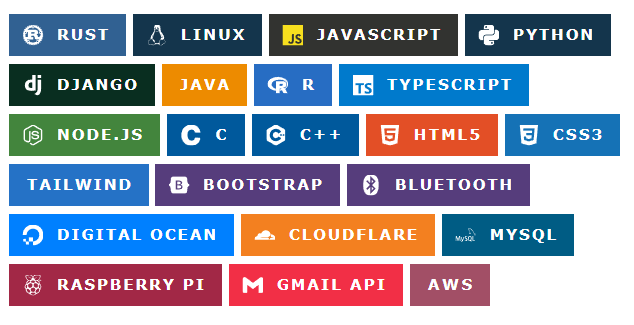
\includegraphics[width=75mm,scale=0.6]{Favorite Technologies.png}}{Rust, Linux, Javascript, Python, Django, Java, R, Typescript, Node.js, C, C++, HTML5, CSS3, Tailwind, Bootstrap, Bluetooth, Digital Ocean, Cloudflare, MySQL, Raspberry PI, Gmail API, AWS}%
